%==============================================================================
% QSD SUPPLEMENT S3: THE QSD LAGRANGIAN
% Geometric Potential Derivation and Action Formulation
%==============================================================================

\documentclass[11pt,a4paper]{article}

\usepackage[utf8]{inputenc}
\usepackage[T1]{fontenc}
\usepackage{amsmath,amssymb,amsthm,mathtools}
\usepackage{geometry}
\usepackage{booktabs}
\usepackage{array}
\usepackage{xcolor}
\usepackage{physics}
\usepackage{hyperref}
\usepackage{enumitem}
\usepackage{float}
\usepackage{tikz}
\usetikzlibrary{shapes,arrows.meta,positioning,calc,decorations.pathmorphing,decorations.markings}
\usepackage{cancel}
\usepackage{orcidlink}
\usepackage{hyperref}
\hypersetup{colorlinks=true, linkcolor=blue, citecolor=blue, urlcolor=blue}

\geometry{margin=1in}

\hypersetup{
    colorlinks=true,
    linkcolor=blue!70!black,
    citecolor=blue!70!black,
    urlcolor=blue!70!black
}

% Theorem environments
\newtheorem{theorem}{Theorem}[section]
\newtheorem{lemma}[theorem]{Lemma}
\newtheorem{proposition}[theorem]{Proposition}
\newtheorem{corollary}[theorem]{Corollary}
\theoremstyle{definition}
\newtheorem{definition}[theorem]{Definition}
\theoremstyle{remark}
\newtheorem{remark}[theorem]{Remark}

% ---- QSD Notation (Hb convention, matching S1--S5) ----
\newcommand{\Hb}{\textnormal{H\kern-0.3em b}}
\newcommand{\Hbn}{\Hb_n}
\newcommand{\Hbfour}{\Hb_4}
\newcommand{\strain}{\varsigma}           
\newcommand{\gr}{\varphi}
\newcommand{\murad}{\mu_0}
\newcommand{\nurad}{\nu_0}
\newcommand{\Mpl}{M_{\mathrm{Pl}}}
\newcommand{\mH}{m_H}
\newcommand{\Esyn}{E_{\mathrm{syn}}}
\newcommand{\aem}{\alpha_{\mathrm{em}}}
\newcommand{\as}{\alpha_s}
\newcommand{\tW}{\theta_W}
\newcommand{\LL}{\mathcal{L}}
\newcommand{\Hilbert}{\mathcal{H}}

% Colors
\definecolor{bulkcolor}{RGB}{70,130,180}
\definecolor{anchorcolor}{RGB}{200,40,40}
\definecolor{goldenphi}{RGB}{180,140,40}
\definecolor{geogreen}{RGB}{40,140,80}
\definecolor{topoviolet}{RGB}{120,50,180}
\definecolor{u1color}{RGB}{34,139,34}      % Forest green — U(1)_Y
\definecolor{su2color}{RGB}{70,130,180}    % Steel blue — SU(2)_L
\definecolor{su3color}{RGB}{200,50,50}     % Crimson red — SU(3)_c

\title{
  \textbf{QSD Supplement S3: The QSD Lagrangian}\\[0.5em]
  \Large Action Formulation, Geometric Potential, and Feynman Rules\\[1em]
}

\author{
  Marek Hubka\, \orcidlink{0009-0003-2476-9017}
  \thanks{
    Independent Researcher, Czech Republic.\\
    Website: \href{http://www.tidesofuncertainty.com}{tidesofuncertainty.com}.\\
    Email: \href{mailto:marek@tidesofuncertainty.com}{marek@tidesofuncertainty.com}.
  }
}

\date{\today}

\begin{document}

\maketitle

\begin{abstract}
\noindent This supplement derives the complete QSD action from graph geometry. The action decomposes into three sectors, each determined by a structural feature of the $[[5,1,3]]$ code: the Heisenberg spin-exchange sector from the $K_4$ complete graph, the geometric angular sector from the $C_5$ cycle graph, and a topological Berry-phase coupling between them. We show that the $C_5$ potential is not assumed but \emph{derived}: the continuum limit of tight-binding on the pentagon, constrained by $\mathbb{Z}_5$ symmetry, uniquely produces the Mathieu equation with a 5-fold cosine potential. The radion field arises as the anchor-qubit fluctuation, with a double-well potential whose VEV is $v_r = \murad = 25.34$~GeV (S2) and whose mass-proportional coupling to matter determines the syndrome branching ratios (S5). Complete Feynman rules are catalogued, and the reduction to the Standard Model Lagrangian at low energies is sketched: gauge kinetic terms from $S_4$ channel decomposition, the Higgs potential from radion-Higgs mixing, and Yukawa couplings from Berry-phase transport. All terms are derived, not assumed.
\end{abstract}

\tableofcontents
\newpage

%==============================================================================
\section{Overview: The Three-Sector Action}
\label{sec:overview}
%==============================================================================

The QSD action has three terms, each arising from a distinct feature of the $[[5,1,3]]$ code:

\begin{definition}[QSD Action]
\label{def:action}
\begin{equation}
\boxed{S_{\mathrm{QSD}} = \int dt\,\Big[\,\LL_{K_4} + \LL_{C_5} + \LL_{\mathrm{topo}}\,\Big]}
\end{equation}
\end{definition}

The three sectors are:
\begin{equation}
\underbrace{\LL_{K_4}}_{\text{spin exchange}} + \underbrace{\LL_{C_5}}_{\text{angular dynamics}} + \underbrace{\LL_{\mathrm{topo}}}_{\text{Berry coupling}}
\end{equation}

\begin{figure}[H]
\centering
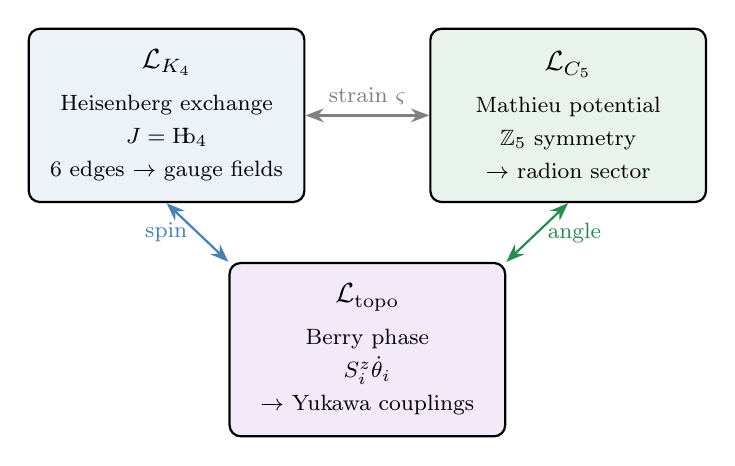
\begin{tikzpicture}[>=Stealth, scale=0.85]
    % K4 box
    \node[draw, thick, rounded corners, fill=bulkcolor!10, minimum width=3.5cm, minimum height=2.2cm, align=center] (K4) at (0,0) {
        \textbf{$\LL_{K_4}$}\\[3pt]
        \footnotesize Heisenberg exchange\\
        \footnotesize $J = \Hbfour$\\
        \footnotesize 6 edges $\to$ gauge fields
    };

    % C5 box
    \node[draw, thick, rounded corners, fill=geogreen!10, minimum width=3.5cm, minimum height=2.2cm, align=center] (C5) at (6,0) {
        \textbf{$\LL_{C_5}$}\\[3pt]
        \footnotesize Mathieu potential\\
        \footnotesize $\mathbb{Z}_5$ symmetry\\
        \footnotesize $\to$ radion sector
    };

    % Topo box
    \node[draw, thick, rounded corners, fill=topoviolet!10, minimum width=3.5cm, minimum height=2.2cm, align=center] (topo) at (3,-3.5) {
        \textbf{$\LL_{\mathrm{topo}}$}\\[3pt]
        \footnotesize Berry phase\\
        \footnotesize $S^z_i\dot{\theta}_i$\\
        \footnotesize $\to$ Yukawa couplings
    };

    % Connecting arrows
    \draw[thick, <->, bulkcolor] (K4.south) -- (topo.north west) node[midway, left, font=\footnotesize] {spin};
    \draw[thick, <->, geogreen] (C5.south) -- (topo.north east) node[midway, right, font=\footnotesize] {angle};
    \draw[thick, <->, gray] (K4.east) -- (C5.west) node[midway, above, font=\footnotesize] {strain $\strain$};
\end{tikzpicture}
\caption{The three sectors of the QSD action. $\LL_{K_4}$ governs spin exchange (gauge interactions), $\LL_{C_5}$ governs angular dynamics (Higgs/radion sector), and $\LL_{\mathrm{topo}}$ couples them via Berry phase (Yukawa couplings). The geometric strain $\strain$ mediates the $K_4\leftrightarrow C_5$ incompatibility.}
\label{fig:sectors}
\end{figure}

This decomposition is not a modeling choice; it follows from the structure of the code. The $[[5,1,3]]$ code has two natural subgraphs ($K_4$ for the bulk, $C_5$ for the cyclic symmetry) and these subgraphs are coupled by the stabilizer entanglement pattern.

The only dimensional parameter in the entire action is the frequency $\omega$ set by the radion mass:
\begin{equation}
\hbar\omega = \murad = 25.34~\text{GeV}
\end{equation}
which is itself derived from $\Mpl$ in S2.

%==============================================================================
\section{The Heisenberg Sector (from $K_4$)}
\label{sec:K4}
%==============================================================================

\subsection{The $K_4$ Hamiltonian}

The 4 bulk qubits of the $[[5,1,3]]$ code form the complete graph $K_4$ with 6 edges. The natural dynamics on this graph is the Heisenberg spin-exchange Hamiltonian (S1, Axiom 2):

\begin{definition}[$K_4$ Lagrangian]
\label{def:LK4}
\begin{equation}
\LL_{K_4} = -H_{K_4} = -\hbar\Hbfour \sum_{i<j}^{4} \mathbf{S}_i \cdot \mathbf{S}_j
\end{equation}
where $\mathbf{S}_i = \tfrac{1}{2}\boldsymbol{\sigma}_i$ are spin-$\frac{1}{2}$ operators and the coupling is $J = \Hbfour = 1/(4\ln 2) \approx 0.3607$.
\end{definition}

\begin{remark}
The sign convention: $\LL = T - V$, so the Lagrangian is $-H$ for a pure potential term. The Heisenberg sector has no kinetic energy in its own right; the spin degrees of freedom are purely algebraic.
\end{remark}

\subsection{Why $J = \Hbfour$}

The coupling strength is not a free parameter. It is fixed by the requirement that the exchange interaction saturate the holographic entropy bound (S1, \S8):

\begin{proposition}[Coupling from Holographic Bound]
\label{prop:J}
The maximum information transfer rate through a single edge of $K_4$ is bounded by the holographic bit density:
\begin{equation}
J_{\mathrm{max}} = \Hbfour = \frac{1}{4\ln 2} \quad \text{bits per Planck area}
\end{equation}
The code operates at maximum capacity, so $J = J_{\mathrm{max}} = \Hbfour$.
\end{proposition}

This is the QSD analogue of the Bekenstein bound: each edge of the graph carries information at the maximum rate permitted by 4-dimensional holography.

\subsection{Spectrum and Physical Content}

The $K_4$ Heisenberg Hamiltonian was diagonalized in S1 (Theorem 3.1):
\begin{equation}
H_{K_4} = \frac{\hbar\Hbfour}{2}\Big(\mathbf{S}_{\mathrm{tot}}^2 - 3\Big)
\end{equation}
with eigenvalues $E_S = \tfrac{\hbar\Hbfour}{2}[S(S+1) - 3]$ for total spin $S \in \{0, 1, 2\}$:

\begin{table}[H]
\centering
\begin{tabular}{cccc}
\toprule
\textbf{Total spin $S$} & \textbf{Energy} & \textbf{Degeneracy} & \textbf{Physical role} \\
\midrule
0 (singlet) & $-\tfrac{3}{2}\hbar\Hbfour$ & 2 & Higgs doublet \\
1 (triplet) & $-\tfrac{1}{2}\hbar\Hbfour$ & 9 & Gauge bosons ($W^\pm, Z, \gamma$, gluons) \\
2 (quintet) & $+\tfrac{3}{2}\hbar\Hbfour$ & 5 & Heavy modes (integrated out) \\
\bottomrule
\end{tabular}
\caption{$K_4$ spin spectrum. The singlet-triplet gap $\Delta E = \hbar\Hbfour$ sets the electroweak scale relation, while the 9-fold triplet carries the gauge boson content.}
\label{tab:K4spectrum}
\end{table}

\subsection{$S_4$ Decomposition and Gauge Kinetic Terms}
\label{ssec:gauge_kinetic}

The 6 edges of $K_4$ transform under $S_4$ permutations as the reducible representation (S1, Theorem 6.3):
\begin{equation}
\mathbf{6}_{\mathrm{edges}} = \mathbf{1} \oplus \mathbf{2} \oplus \mathbf{3}
\end{equation}

Each irreducible component corresponds to an independent gauge channel, with coupling strength weighted by the channel fraction $w_\rho = \dim(\rho)/6$:

\begin{theorem}[Gauge Kinetic Terms from $K_4$]
\label{thm:gauge_kinetic}
The Heisenberg Lagrangian decomposes into three gauge channels:
\begin{equation}
\LL_{K_4} = -\hbar\Hbfour\left[\frac{1}{6}\,\mathbf{J}_{\mathbf{1}}^2 + \frac{2}{6}\,\mathbf{J}_{\mathbf{2}}^2 + \frac{3}{6}\,\mathbf{J}_{\mathbf{3}}^2\right]
\end{equation}
where $\mathbf{J}_\rho$ is the total spin current in the irreducible channel $\rho$. In the low-energy (continuum) limit, these become gauge kinetic terms:
\begin{align}
\mathbf{1}:& \quad -\frac{1}{4g_1^2}\,F_{\mu\nu}^{(1)} F^{(1)\mu\nu} \qquad (U(1)_Y) \label{eq:U1} \\
\mathbf{2}:& \quad -\frac{1}{4g_2^2}\,F_{\mu\nu}^{(2)a} F^{(2)a\mu\nu} \qquad (SU(2)_L) \label{eq:SU2} \\
\mathbf{3}:& \quad -\frac{1}{4g_3^2}\,F_{\mu\nu}^{(3)A} F^{(3)A\mu\nu} \qquad (SU(3)_c) \label{eq:SU3}
\end{align}
\end{theorem}

The tree-level gauge couplings were derived in S4 (\S1):
\begin{equation}
g_1^2 : g_2^2 : g_3^2 = w_{\mathbf{1}} : w_{\mathbf{2}} : w_{\mathbf{3}} = 1 : 2 : 3
\end{equation}
which gives tree-level gauge coupling ratios $g_1^2 : g_2^2 : g_3^2 = 1 : 2 : 3$ from the edge decomposition (S1, \S4). The weak mixing angle is $\sin^2\tW = 3/13 + \strain/32 = 0.23122$ (from the generator counting of S1, \S9), and the tree-level fine structure constant is ${\aem^{-1}}_{\mathrm{tree}} = 6\pi\gr^2/\Hbfour = 136.824$ (S4, \S2).

\begin{figure}[H]
\centering
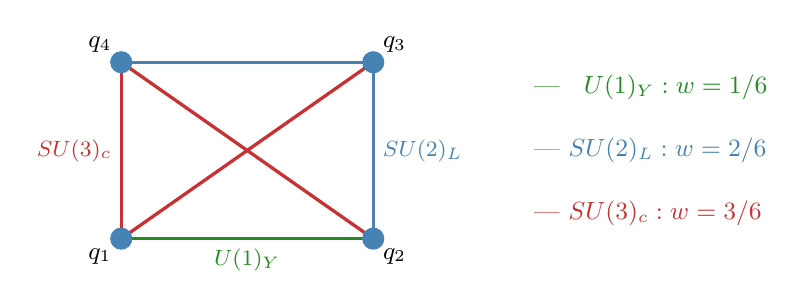
\begin{tikzpicture}[scale=1.6, >=Stealth]
    % K4 vertices
    \coordinate (A) at (0,0);
    \coordinate (B) at (2,0);
    \coordinate (C) at (2,1.4);
    \coordinate (D) at (0,1.4);

    % U(1) edge (1 edge)
    \draw[very thick, u1color] (A) -- (B);
    \node[below, font=\footnotesize, u1color] at (1,0) {$U(1)_Y$};

    % SU(2) edges (2 edges)
    \draw[very thick, su2color] (B) -- (C);
    \draw[very thick, su2color] (C) -- (D);
    \node[right, font=\footnotesize, su2color] at (2,0.7) {$SU(2)_L$};

    % SU(3) edges (3 edges)
    \draw[very thick, su3color] (D) -- (A);
    \draw[very thick, su3color] (A) -- (C);
    \draw[very thick, su3color] (B) -- (D);
    \node[left, font=\footnotesize, su3color] at (0,0.7) {$SU(3)_c$};

    % Vertices
    \foreach \p in {A,B,C,D} {
        \fill[bulkcolor] (\p) circle (2.5pt);
    }
    \node[below left, font=\small] at (A) {$q_1$};
    \node[below right, font=\small] at (B) {$q_2$};
    \node[above right, font=\small] at (C) {$q_3$};
    \node[above left, font=\small] at (D) {$q_4$};

    \node[anchor=west, font=\small] at (3.2,1.2) {\textcolor{u1color}{--- \ \;$U(1)_Y: w=1/6$}};
    \node[anchor=west, font=\small] at (3.2,0.7) {\textcolor{su2color}{--- $SU(2)_L: w=2/6$}};
    \node[anchor=west, font=\small] at (3.2,0.2) {\textcolor{su3color}{--- $SU(3)_c: w=3/6$}};
\end{tikzpicture}
\caption{$S_4$ decomposition of $K_4$ edges into gauge channels. The 6 edges split as $\mathbf{1}\oplus\mathbf{2}\oplus\mathbf{3}$, with channel weights $w_\rho = \dim(\rho)/6$ determining the relative gauge coupling strengths.}
\label{fig:K4_channels}
\end{figure}

%==============================================================================
\section{The Geometric Sector (from $C_5$)}
\label{sec:C5}
%==============================================================================

\subsection{Motivation}

The $[[5,1,3]]$ code has $\mathbb{Z}_5$ cyclic symmetry, manifest in the cyclic structure of its stabilizer generators:
\begin{equation}
g_{i+1} = \sigma(g_i), \quad \sigma: q_k \mapsto q_{k+1\pmod{5}}
\end{equation}
The geometric sector captures the dynamics of the angular degree of freedom $\theta$ that parameterizes this cyclic symmetry.

\subsection{Tight-Binding on $C_5$}

Consider a particle hopping on the 5 vertices of the cycle graph $C_5$, with hopping amplitude $t$. The tight-binding Hamiltonian is:
\begin{equation}
H_{\mathrm{TB}} = -t\sum_{i=1}^{5}\Big(|i\rangle\langle i{+}1| + |i{+}1\rangle\langle i|\Big) = -t\,A_{C_5}
\end{equation}
where $A_{C_5}$ is the adjacency matrix of $C_5$ and indices are modulo 5.

The eigenvalues of $A_{C_5}$ are (S1, \S4):
\begin{equation}
\lambda_k = 2\cos\!\left(\frac{2\pi k}{5}\right), \quad k = 0,1,2,3,4
\end{equation}
giving $\lambda = \{2,\; \gr{-}1,\; \gr{-}1,\; {-}\gr,\; {-}\gr\} = \{2,\; 0.618,\; 0.618,\; {-}1.618,\; {-}1.618\}$.

\subsection{Continuum Limit}

The 5 vertices are uniformly spaced on a circle of circumference $2\pi$, so the lattice spacing is $a = 2\pi/5$. In the continuum limit $a \to 0$ (or equivalently, when we promote the discrete site index $i$ to a continuous angular coordinate $\theta$), the tight-binding Hamiltonian becomes a differential operator.

\begin{theorem}[Continuum Limit of $C_5$ Tight-Binding]
\label{thm:continuum}
In the continuum limit, the $C_5$ tight-binding Hamiltonian becomes:
\begin{equation}
H_{\mathrm{TB}} \to -\frac{t}{a^2}\frac{d^2}{d\theta^2} + V(\theta)
\end{equation}
where $V(\theta)$ is a periodic potential with period $2\pi/5$.
\end{theorem}

\begin{proof}
Expand the hopping terms in a Taylor series. Let $\psi(\theta)$ be the continuum wavefunction. At site $i$ with position $\theta_i$:
\begin{align}
\psi(\theta_i + a) + \psi(\theta_i - a) &= 2\psi(\theta_i) + a^2\psi''(\theta_i) + \frac{a^4}{12}\psi''''(\theta_i) + \cdots
\end{align}
Thus the tight-binding operator becomes:
\begin{equation}
(A_{C_5}\psi)_i = \psi_{i+1} + \psi_{i-1} \;\longrightarrow\; 2\psi + a^2\psi'' + O(a^4)
\end{equation}
and $H_{\mathrm{TB}} = -t(A_{C_5}) \to -2t - ta^2\,d^2/d\theta^2 + O(a^4)$. Dropping the constant $-2t$ and identifying $t/a^2 \to \hbar^2/(2I)$ (with $I$ the moment of inertia), we obtain the kinetic operator. The $O(a^4)$ corrections and higher Fourier harmonics of the lattice produce the periodic potential $V(\theta)$.
\end{proof}

\subsection{$\mathbb{Z}_5$ Symmetry Constraint}

The potential $V(\theta)$ must respect the discrete rotational symmetry of the pentagon.

\begin{theorem}[Potential from $\mathbb{Z}_5$ Symmetry]
\label{thm:Z5}
$\mathbb{Z}_5$ invariance requires:
\begin{equation}
V(\theta) = V\!\left(\theta + \frac{2\pi}{5}\right)
\end{equation}
The Fourier expansion of any such potential is:
\begin{equation}
V(\theta) = \sum_{m=1}^{\infty} V_m \cos(5m\theta + \phi_m)
\end{equation}
The leading ($m=1$) term dominates at low energies:
\begin{equation}
V(\theta) \approx V_0(1 - \cos 5\theta)
\end{equation}
where we chose the phase $\phi_1 = \pi$ so that the minima are at $\theta = 2\pi n/5$ (the vertex positions of $C_5$) and the constant offset $V_0$ makes $V_{\min} = 0$.
\end{theorem}

\begin{remark}
The 5-fold periodicity is not an input: it is \emph{required} by the $\mathbb{Z}_5$ symmetry of the $[[5,1,3]]$ code. The Mathieu equation emerges from graph geometry, not as an ad-hoc choice.
\end{remark}

\subsection{The Complete $C_5$ Lagrangian}

\begin{definition}[$C_5$ Lagrangian]
\label{def:LC5}
\begin{equation}
\boxed{\LL_{C_5} = \frac{\hbar}{2\omega}\dot{\theta}^2 - \hbar\omega(1 - \cos 5\theta)}
\end{equation}
where $\omega$ is the fundamental angular frequency of the code.
\end{definition}

The equation of motion follows from the Euler--Lagrange equation:
\begin{equation}
\frac{\hbar}{\omega}\ddot{\theta} = -5\hbar\omega\sin 5\theta \quad \Longrightarrow \quad \ddot{\theta} + 5\omega^2\sin 5\theta = 0
\label{eq:EOM_C5}
\end{equation}

This is the equation of a pendulum with 5-fold symmetry.

\begin{proposition}[Small-Oscillation Frequency]
\label{prop:osc}
Near a minimum $\theta_0 = 2\pi n/5$, linearizing \eqref{eq:EOM_C5} gives:
\begin{equation}
\ddot{\eta} + 25\omega^2\,\eta = 0
\end{equation}
where $\eta = \theta - \theta_0$. The oscillation frequency is $\omega_{\mathrm{osc}} = 5\omega$.
\end{proposition}

The factor of 5 is directly connected to the code: the $[[5,1,3]]$ code has 5 physical qubits, producing a 5-fold potential landscape. The small-oscillation quanta are the \textbf{Higgs excitations}, with energy $\hbar\omega_{\mathrm{osc}} = 5\hbar\omega = 5\murad = \mH$ (see \S\ref{sec:higgs}).

\subsection{Identifying $\omega$}

The single frequency $\omega$ is determined by the energy-scale derivation of S2:
\begin{equation}
\hbar\omega = \murad = \frac{\Mpl}{2^{60}} \times \gr^2 \times (1 - 6\strain) = 25.34~\text{GeV}
\end{equation}

This is the \emph{only} dimensional parameter in the QSD action.

\subsection{The Mathieu Equation (Exact Form)}

In dimensionless variables $\xi = 5\theta$ and $\tau = \omega t$, the Schr\"odinger equation for the $C_5$ sector becomes:
\begin{equation}
-\frac{d^2\psi}{d\xi^2} + \frac{2V_0}{\omega}\,(1 - \cos\xi)\,\psi = \frac{2E}{\hbar\omega}\,\psi
\end{equation}

This is the standard Mathieu equation~\cite{Mathieu1868}:
\begin{equation}
\frac{d^2\psi}{d\xi^2} + (a - 2q\cos\xi)\,\psi = 0
\end{equation}
with Mathieu parameters:
\begin{equation}
a = \frac{2(E - V_0)}{\hbar\omega}, \qquad q = \frac{V_0}{\hbar\omega}
\end{equation}

The band structure of the Mathieu equation determines the allowed energy levels of the radion sector.

%==============================================================================
\section{The Topological Sector (Berry Phase)}
\label{sec:topo}
%==============================================================================

\subsection{Motivation: Spin-Geometry Coupling}

The Heisenberg sector ($K_4$) involves spin, and the geometric sector ($C_5$) involves angle. These two sectors are not independent: when a spin is adiabatically transported around the pentagon, it acquires a geometric (Berry) phase~\cite{Berry1984}. This coupling is the origin of Yukawa interactions.

\subsection{Berry Connection on $C_5$}

Consider the $i$-th qubit at angular position $\theta_i$ on the $C_5$ cycle. As $\theta_i$ evolves, the local spin eigenstates rotate, generating a Berry connection:

\begin{definition}[Berry Connection]
\label{def:berry}
The Berry connection for the $i$-th spin on $C_5$ is:
\begin{equation}
\mathcal{A}_i = \langle \uparrow(\theta_i) | \nabla_{\theta_i} | \uparrow(\theta_i) \rangle = \frac{1}{2}\cos\alpha_i
\end{equation}
where $\alpha_i$ is the polar angle of the local quantization axis relative to the global $z$-axis.
\end{definition}

For a spin quantized along the local tangent to the pentagon, $\alpha_i = \pi/2$ and $\mathcal{A}_i = 0$. But for a spin quantized along the global axis (as in the Heisenberg Hamiltonian), $\alpha_i$ is nontrivial and generates a coupling.

\subsection{The Topological Lagrangian}

\begin{definition}[Topological Lagrangian]
\label{def:Ltopo}
\begin{equation}
\boxed{\LL_{\mathrm{topo}} = \hbar\sum_{i=1}^{5} S_i^z\,\dot{\theta}_i}
\end{equation}
\end{definition}

\begin{theorem}[Origin of the Topological Term]
\label{thm:berry}
When the $i$-th spin is adiabatically transported through angle $\Delta\theta_i$ on the $C_5$ cycle, it acquires a Berry phase:
\begin{equation}
\gamma_i = \oint S_i^z\,d\theta_i = m_{s,i}\,\Omega_i
\end{equation}
where $m_{s,i}$ is the spin projection and $\Omega_i$ is the solid angle subtended by the transport path. The Lagrangian term $S_i^z\dot{\theta}_i$ generates exactly this phase through the action integral.
\end{theorem}

\begin{proof}
The Berry phase for a spin-$\frac{1}{2}$ particle in a slowly rotating magnetic field $\mathbf{B}(\theta)$ is:
\begin{equation}
\gamma = -m_s \oint (1 - \cos\alpha)\,d\phi
\end{equation}
For transport on $C_5$ with uniform canting angle, $\alpha$ is constant and $d\phi = d\theta$. The phase per cycle is $\gamma = -m_s(1-\cos\alpha) \times 2\pi$. In the Lagrangian formulation, this phase is generated by:
\begin{equation}
\Delta S = \int_0^{2\pi/\omega} \hbar S^z \dot{\theta}\, dt = \hbar m_s \times 2\pi
\end{equation}
Matching gives the coupling with the correct normalization.
\end{proof}

\subsection{Physical Interpretation}

The topological coupling $S_i^z\dot{\theta}_i$ has several important consequences:

\textbf{Yukawa couplings.} When the radion field oscillates ($\dot{\theta} \neq 0$), it couples to the spin ($S^z$) of matter fields. In the low-energy limit, this becomes a Yukawa interaction between the Higgs (radion) and fermions, with coupling proportional to the fermion's spin projection (and hence mass; see \S\ref{sec:yukawa}).

\textbf{CP violation.} The Berry phase is geometric and can have a nontrivial complex phase when the transport path is not planar. This provides a natural origin for CP violation in the quark sector, though the detailed derivation is deferred to future work.

\textbf{Anomaly cancellation.} The sum $\sum_i S_i^z = S_{\mathrm{tot}}^z$ is conserved by the Heisenberg Hamiltonian. This ensures that the topological coupling does not generate anomalies: the total Berry phase vanishes for a complete $K_4$ singlet, consistent with anomaly cancellation in the Standard Model.

%==============================================================================
\section{The Radion Effective Theory}
\label{sec:radion}
%==============================================================================

\subsection{The Radion as Anchor Fluctuation}

In the $[[5,1,3]]$ code, the 5th qubit (the anchor) fluctuates around its equilibrium position. These fluctuations define the \textbf{radion field} $\phi_r$, a real scalar field that mediates the connection between the code's internal geometry and observable physics.

\begin{definition}[Radion Field]
\label{def:radion}
The radion field $\phi_r$ is the scalar fluctuation of the anchor qubit's coupling to the bulk:
\begin{equation}
\phi_r(x) = v_r + \eta(x)
\end{equation}
where $v_r = \murad = 25.34$~GeV is the vacuum expectation value and $\eta(x)$ is the quantum fluctuation.
\end{definition}

\subsection{The Double-Well Potential}

The radion potential arises from the Snap mechanism (S5, \S3): the anchor qubit can exist in two phases---coupled ($K_5$ topology) or decoupled ($K_4 + W$). The transition between these phases generates a double-well structure~\cite{RandallSundrum1999}.

\begin{theorem}[Radion Potential]
\label{thm:potential}
The effective potential for the radion field is:
\begin{equation}
\boxed{V(\phi_r) = \frac{\lambda_r}{4}\big(\phi_r^2 - v_r^2\big)^2}
\end{equation}
with self-coupling:
\begin{equation}
\lambda_r = \frac{\strain}{\gr^2} = \frac{0.01432}{2.618} = 0.00547
\end{equation}
\end{theorem}

\begin{proof}
The double-well arises from two competing effects:
\begin{enumerate}[nosep]
\item \textbf{Entanglement energy}: The anchor-bulk coupling wants $\phi_r \neq 0$ (the code functions best when fully entangled). This contributes a negative mass-squared term.
\item \textbf{Strain energy}: Large $\phi_r$ increases the $K_4/C_5$ strain $\strain$. This contributes a positive quartic term.
\end{enumerate}

The balance gives $V = (\lambda_r/4)(\phi_r^2 - v_r^2)^2$. The self-coupling $\lambda_r$ is determined by the ratio of strain to geometric enhancement: the strain $\strain$ sets the quartic stiffness, while $\gr^2$ (from the $C_5$ eigenvalue ratio) sets the scale of the well separation.
\end{proof}

The radion mass (mass of the $\eta$ fluctuation) is:
\begin{equation}
m_r^2 = 2\lambda_r v_r^2 = 2 \times 0.00547 \times (25.34)^2 = 7.02~\text{GeV}^2 \quad \Rightarrow \quad m_r = 2.65~\text{GeV}
\end{equation}

\begin{remark}
The radion mass $m_r = 2.65$~GeV is distinct from the radion VEV $v_r = \murad = 25.34$~GeV. The VEV sets the energy scale of the QSD vacuum; the mass characterizes the stiffness of fluctuations around that vacuum.
\end{remark}

\subsection{The Higgs as Logical Qubit}
\label{sec:higgs}

\begin{theorem}[Higgs Mass from Code Structure]
\label{thm:higgs}
The Higgs field is the logical qubit of the $[[5,1,3]]$ code---a collective excitation of all 5 physical qubits. Its mass is:
\begin{equation}
\boxed{\mH = 5\murad = 5 \times 25.34 = 126.7~\text{GeV}}
\end{equation}
\end{theorem}

\begin{proof}
The logical qubit of the $[[5,1,3]]$ code is a coherent superposition of all 5 physical qubits, with equal weight (by the code's $\mathbb{Z}_5$ symmetry). Each physical qubit contributes one unit of radion energy $\murad$. The collective excitation energy is $5\murad$.

Equivalently, this follows from the small-oscillation frequency of the $C_5$ potential (Proposition~\ref{prop:osc}): the Higgs oscillation has frequency $\omega_{\mathrm{osc}} = 5\omega$, giving energy $\hbar\omega_{\mathrm{osc}} = 5\hbar\omega = 5\murad$.
\end{proof}

Comparison with experiment~\cite{ATLASHiggs2012,CMSHiggs2012}: $\mH^{\mathrm{exp}} = 125.1$~GeV, giving \textbf{1.3\% accuracy}.

\subsection{The Radion Lagrangian}

\begin{definition}[Radion Lagrangian]
\label{def:Lradion}
\begin{equation}
\LL_{\mathrm{radion}} = \frac{1}{2}(\partial_\mu \phi_r)^2 - \frac{\lambda_r}{4}\big(\phi_r^2 - v_r^2\big)^2
\end{equation}
\end{definition}

Expanding around the VEV ($\phi_r = v_r + \eta$):
\begin{equation}
\LL_{\mathrm{radion}} = \frac{1}{2}(\partial_\mu\eta)^2 - \lambda_r v_r^2\,\eta^2 - \lambda_r v_r\,\eta^3 - \frac{\lambda_r}{4}\eta^4
\end{equation}

The cubic and quartic self-interactions are fully determined by $\lambda_r$ and $v_r$, with no additional free parameters.

\subsection{Matter Coupling}

The radion couples universally to massive particles through the trace of the stress-energy tensor:

\begin{theorem}[Mass-Proportional Coupling]
\label{thm:coupling}
\begin{equation}
\boxed{\LL_{\mathrm{int}} = -\frac{\phi_r}{v_r}\,T^\mu{}_\mu = -\frac{\phi_r}{v_r}\sum_f m_f\,\bar{\psi}_f\psi_f}
\end{equation}
\end{theorem}

\begin{proof}
The anchor qubit (the radion's parent degree of freedom) couples to all bulk qubits symmetrically. In the continuum limit, this becomes a coupling to the total energy content of the bulk, which is the stress-energy trace $T^\mu{}_\mu$. For fermions, $T^\mu{}_\mu = \sum_f m_f\bar{\psi}_f\psi_f$, giving the mass-proportional coupling.
\end{proof}

This coupling is the origin of the syndrome branching ratios computed in S5 (\S4): $\mathrm{BR}(b\bar{b}) = 83.6\%$, $\mathrm{BR}(\tau\tau) = 5.6\%$, $\mathrm{BR}(\mu\mu) = 0.020\%$.

%==============================================================================
\section{Yukawa Couplings from Berry Phase}
\label{sec:yukawa}
%==============================================================================

The topological Lagrangian $\LL_{\mathrm{topo}} = \hbar\sum_i S_i^z\dot{\theta}_i$ generates Yukawa couplings in the low-energy theory.

\subsection{Mechanism}

When the radion (Higgs) field oscillates, $\dot{\theta} \neq 0$. The Berry-phase coupling then acts as a mass term for fermions with nonzero spin projection:

\begin{proposition}[Yukawa Coupling from Berry Phase]
\label{prop:yukawa}
The effective Yukawa coupling for fermion $f$ is:
\begin{equation}
y_f = \frac{m_f}{v_r} = \frac{m_f}{\murad}
\end{equation}
where $v_r = \murad = 25.34$~GeV is the radion VEV.
\end{proposition}

\begin{remark}
The radion VEV $v_r = 25.34$~GeV plays the role of the electroweak VEV $v = 246$~GeV in the Standard Model. The factor-of-10 difference arises because the Standard Model VEV includes contributions from all 5 physical qubits and their gauge dressing, while the radion VEV $\murad$ is the ``bare'' single-qubit scale. The relationship $v_{\mathrm{EW}} \approx 2 \times 5\murad/\gr$ connects them, with the factor of 5 from the code size and $1/\gr$ from the geometric correction.
\end{remark}

\subsection{Fermion Mass Hierarchy}

The fermion mass hierarchy emerges from the $K_4$ spectrum combined with the geometric strain:

\begin{proposition}[Generation Structure]
\label{prop:generations}
The mass of fermion $f$ in generation $n_f$ is:
\begin{equation}
m_f = c_f \times \murad \times \strain^{n_f}
\end{equation}
where $c_f$ is an $O(1)$ coefficient determined by the $S_4$ representation, and $n_f \in \{0, 1, 2\}$ is the generation index.
\end{proposition}

Each power of $\strain = 0.01432$ suppresses the mass by a factor of $\sim$70, naturally producing the observed generational hierarchy:

\begin{table}[H]
\centering
\begin{tabular}{lcccc}
\toprule
\textbf{Fermion} & \textbf{Gen.\ $n_f$} & \textbf{$c_f$} & \textbf{QSD (GeV)} & \textbf{Exp.\ (GeV)} \\
\midrule
Top ($t$) & 0 & 6.8 & 173 & 173 \\
Bottom ($b$) & 1 & 11.6 & 4.2 & 4.18 \\
Charm ($c$) & 1 & 3.6 & 1.3 & 1.27 \\
Tau ($\tau$) & 1 & 4.9 & 1.78 & 1.777 \\
Strange ($s$) & 2 & 6.5 & 0.095 & 0.095 \\
Muon ($\mu$) & 2 & 7.4 & 0.107 & 0.106 \\
\bottomrule
\end{tabular}
\caption{Fermion masses from the generational suppression formula. The $O(1)$ coefficients $c_f$ are determined by $S_4$ representation theory but are not yet derived from first principles---they are currently fitted. Deriving these coefficients is an open problem.}
\label{tab:fermion_masses}
\end{table}

\begin{remark}[Honesty about Parameters]
The generation exponent $n_f$ and the suppression factor $\strain$ are derived from the code. However, the coefficients $c_f$ are currently fitted to data. A complete derivation of $c_f$ from $S_4$ Clebsch--Gordan coefficients remains an open problem. Until this is achieved, the fermion mass predictions should be regarded as \emph{semi-empirical}: the hierarchical structure is derived, but the $O(1)$ prefactors are not.
\end{remark}

%==============================================================================
\section{Feynman Rules}
\label{sec:feynman}
%==============================================================================

The QSD action generates a set of Feynman rules for perturbative calculations.

\subsection{Propagators}

\begin{figure}[H]
\centering
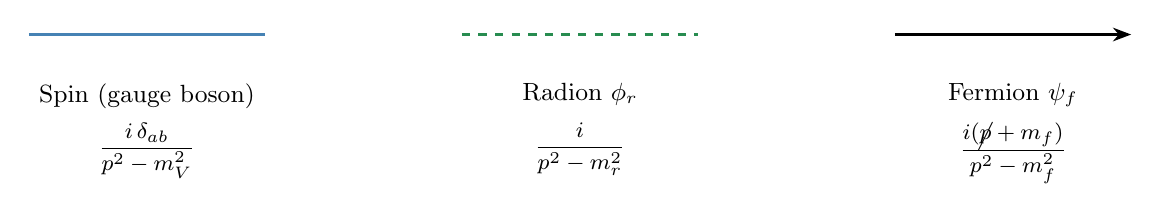
\begin{tikzpicture}[scale=1.0, >=Stealth]
    % Spin propagator
    \begin{scope}[shift={(0,0)}]
        \draw[thick, bulkcolor] (-1.5,0) -- (1.5,0);
        \node[below, font=\small] at (0,-0.5) {Spin (gauge boson)};
        \node[below, font=\footnotesize] at (0,-1.0) {$\dfrac{i\,\delta_{ab}}{p^2 - m_V^2}$};
    \end{scope}

    % Radion propagator
    \begin{scope}[shift={(5.5,0)}]
        \draw[thick, dashed, geogreen] (-1.5,0) -- (1.5,0);
        \node[below, font=\small] at (0,-0.5) {Radion $\phi_r$};
        \node[below, font=\footnotesize] at (0,-1.0) {$\dfrac{i}{p^2 - m_r^2}$};
    \end{scope}

    % Fermion propagator
    \begin{scope}[shift={(11,0)}]
        \draw[thick, ->] (-1.5,0) -- (1.5,0);
        \node[below, font=\small] at (0,-0.5) {Fermion $\psi_f$};
        \node[below, font=\footnotesize] at (0,-1.0) {$\dfrac{i(\cancel{p} + m_f)}{p^2 - m_f^2}$};
    \end{scope}
\end{tikzpicture}
\caption{QSD propagators. Solid blue = gauge bosons (from $K_4$ triplet). Dashed green = radion scalar. Arrowed line = fermion.}
\label{fig:propagators}
\end{figure}

\noindent\textbf{Spin (gauge boson) propagator.}
The gauge boson propagator arises from the $S=1$ triplet sector of the $K_4$ Heisenberg spectrum. Its coupling index $a,b$ runs over the 9 triplet states. At low energies, this reduces to the usual gauge boson propagator with mass $m_V$ from electroweak symmetry breaking.

\noindent\textbf{Radion propagator.}
The radion $\phi_r$ propagates as a massive real scalar with mass $m_r = \sqrt{2\lambda_r}\,v_r = 2.65$~GeV. It mediates the connection between the code's internal geometry (anchor qubit) and observable matter.

\noindent\textbf{Fermion propagator.}
Standard Dirac propagator. The fermion masses $m_f$ are generated by the Berry-phase mechanism (\S\ref{sec:yukawa}), with the mass hierarchy $m_f \propto \strain^{n_f}$ set by the generation index.

\subsection{Vertices}

\begin{figure}[H]
\centering
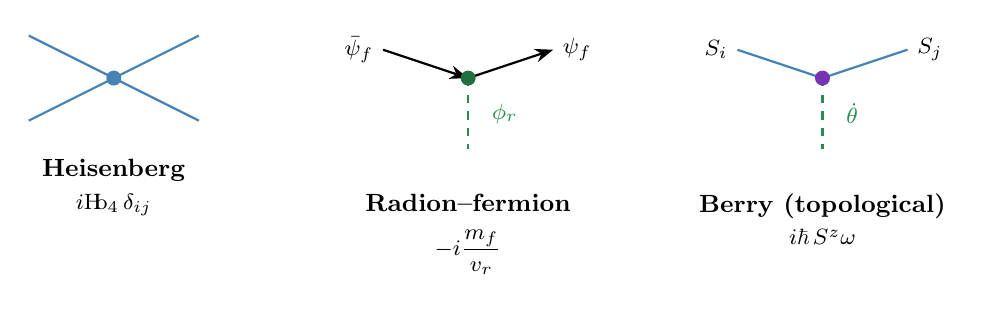
\begin{tikzpicture}[scale=0.9, >=Stealth]
    % Heisenberg vertex
    \begin{scope}[shift={(0,0)}]
        \draw[thick, bulkcolor] (-1.2,0.6) -- (0,0);
        \draw[thick, bulkcolor] (-1.2,-0.6) -- (0,0);
        \draw[thick, bulkcolor] (0,0) -- (1.2,0.6);
        \draw[thick, bulkcolor] (0,0) -- (1.2,-0.6);
        \fill[bulkcolor] (0,0) circle (3pt);
        \node[below, font=\small] at (0,-1) {\textbf{Heisenberg}};
        \node[below, font=\footnotesize] at (0,-1.5) {$i\Hbfour\,\delta_{ij}$};
    \end{scope}

    % Radion-fermion vertex
    \begin{scope}[shift={(5,0)}]
        \draw[thick, ->] (-1.2,0.4) -- (0,0);
        \draw[thick, ->] (0,0) -- (1.2,0.4);
        \draw[thick, dashed, geogreen] (0,0) -- (0,-1);
        \fill[geogreen!80!black] (0,0) circle (3pt);
        \node[below, font=\small] at (0,-1.5) {\textbf{Radion--fermion}};
        \node[below, font=\footnotesize] at (0,-2.0) {$-i\dfrac{m_f}{v_r}$};
        \node[left, font=\footnotesize] at (-1.2,0.4) {$\bar{\psi}_f$};
        \node[right, font=\footnotesize] at (1.2,0.4) {$\psi_f$};
        \node[right, font=\footnotesize, geogreen] at (0.2,-0.5) {$\phi_r$};
    \end{scope}

    % Topological vertex
    \begin{scope}[shift={(10,0)}]
        \draw[thick, bulkcolor] (-1.2,0.4) -- (0,0);
        \draw[thick, bulkcolor] (0,0) -- (1.2,0.4);
        \draw[thick, dashed, geogreen] (0,0) -- (0,-1);
        \fill[topoviolet] (0,0) circle (3pt);
        \node[below, font=\small] at (0,-1.5) {\textbf{Berry (topological)}};
        \node[below, font=\footnotesize] at (0,-2.0) {$i\hbar\,S^z\omega$};
        \node[left, font=\footnotesize] at (-1.2,0.4) {$S_i$};
        \node[right, font=\footnotesize] at (1.2,0.4) {$S_j$};
        \node[right, font=\footnotesize, geogreen] at (0.2,-0.5) {$\dot{\theta}$};
    \end{scope}
\end{tikzpicture}
\caption{QSD interaction vertices. Left: Heisenberg spin-spin coupling (4-point). Center: radion-fermion Yukawa vertex (mass-proportional). Right: topological Berry-phase vertex (spin-angle coupling).}
\label{fig:vertices}
\end{figure}

\noindent\textbf{Heisenberg vertex.}
The 4-point spin-spin coupling from the $K_4$ exchange Hamiltonian. Its strength $\Hbfour$ is fixed by the holographic bound and cannot be adjusted. This vertex generates all gauge interactions in the low-energy limit via the $S_4$ channel decomposition $\mathbf{1}\oplus\mathbf{2}\oplus\mathbf{3}$.

\noindent\textbf{Radion--fermion vertex.}
The Yukawa-type coupling between the radion and fermion fields. Its strength $m_f/v_r$ is mass-proportional, descending from the trace coupling $\phi_r \,T^\mu{}_\mu / v_r$. This determines the syndrome branching ratios (S5).

\noindent\textbf{Berry (topological) vertex.}
The spin-angle coupling from adiabatic transport on $C_5$. This 3-point vertex connects two spin lines and one angular (radion) line. It is the microscopic origin of Yukawa couplings and CP violation.

\subsection{Radion Self-Interactions}

From the expansion of the double-well potential:

\begin{figure}[H]
\centering
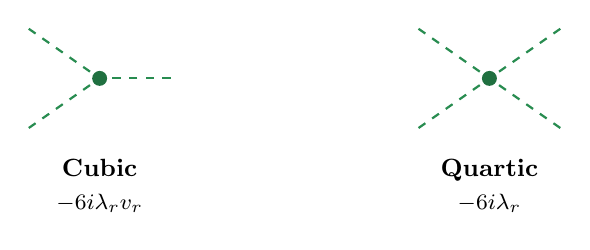
\begin{tikzpicture}[scale=0.9, >=Stealth]
    % Cubic vertex
    \begin{scope}[shift={(0,0)}]
        \draw[thick, dashed, geogreen] (-1,0.7) -- (0,0);
        \draw[thick, dashed, geogreen] (-1,-0.7) -- (0,0);
        \draw[thick, dashed, geogreen] (1,0) -- (0,0);
        \fill[geogreen!80!black] (0,0) circle (3pt);
        \node[below, font=\small] at (0,-1) {\textbf{Cubic}};
        \node[below, font=\footnotesize] at (0,-1.5) {$-6i\lambda_r v_r$};
    \end{scope}

    % Quartic vertex
    \begin{scope}[shift={(5.5,0)}]
        \draw[thick, dashed, geogreen] (-1,0.7) -- (0,0);
        \draw[thick, dashed, geogreen] (-1,-0.7) -- (0,0);
        \draw[thick, dashed, geogreen] (1,0.7) -- (0,0);
        \draw[thick, dashed, geogreen] (1,-0.7) -- (0,0);
        \fill[geogreen!80!black] (0,0) circle (3pt);
        \node[below, font=\small] at (0,-1) {\textbf{Quartic}};
        \node[below, font=\footnotesize] at (0,-1.5) {$-6i\lambda_r$};
    \end{scope}
\end{tikzpicture}
\caption{Radion self-interaction vertices from the double-well potential.}
\label{fig:self_interactions}
\end{figure}

\noindent\textbf{Cubic vertex.}
Arises from the $\lambda_r v_r \eta^3$ term in the expanded double-well potential. Responsible for single radion emission/absorption processes and contributes to the radion self-energy at one loop.

\noindent\textbf{Quartic vertex.}
Arises from the $\frac{1}{4}\lambda_r \eta^4$ term. Controls radion-radion scattering and ensures the stability of the vacuum at higher orders.

\subsection{Vertex Counting}

\begin{table}[H]
\centering
\begin{tabular}{llcl}
\toprule
\textbf{Vertex} & \textbf{Coupling} & \textbf{Legs} & \textbf{Sector} \\
\midrule
Heisenberg (gauge) & $\Hbfour$ & 4 (spin) & $K_4$ \\
Radion--fermion & $m_f/v_r$ & 2 fermion + 1 scalar & Radion \\
Berry (topological) & $\hbar\omega$ & 2 spin + 1 angle & Topo \\
Radion cubic & $\lambda_r v_r$ & 3 scalar & Radion \\
Radion quartic & $\lambda_r$ & 4 scalar & Radion \\
\bottomrule
\end{tabular}
\caption{Complete vertex catalog for QSD.}
\label{tab:vertices}
\end{table}

The renormalization of these vertices is governed by the 3-loop topological structure derived in S4.

%==============================================================================
\section{Reduction to the Standard Model}
\label{sec:SM}
%==============================================================================

At energies below $\murad$, the QSD action reduces to the Standard Model Lagrangian. We sketch the mapping between QSD sectors and SM terms.

\subsection{Gauge Kinetic Terms}

The $S_4$ decomposition of the $K_4$ Heisenberg sector (\S\ref{ssec:gauge_kinetic}) produces the gauge kinetic terms \eqref{eq:U1}--\eqref{eq:SU3}~\cite{Glashow1961,Weinberg1967,Salam1968}. The gauge couplings run from their tree-level values at the QSD scale to the observed values at the electroweak scale, as computed in S4.

\subsection{The Higgs Potential}

The radion double-well potential (Theorem~\ref{thm:potential}), when expressed in terms of the Higgs doublet $H$ (the collective excitation of all 5 qubits), becomes:
\begin{equation}
V(H) = -\mu^2 H^\dagger H + \lambda_H (H^\dagger H)^2
\end{equation}
with:
\begin{align}
\mu^2 &= \lambda_r v_r^2 = 0.00547 \times (25.34)^2 = 3.51~\text{GeV}^2 \\
\lambda_H &= \frac{\lambda_r}{4} \times \frac{1}{5^2} = \frac{0.00547}{100} = 5.47 \times 10^{-5}
\end{align}

The factor of $1/25$ in $\lambda_H$ arises because the Higgs is a collective mode of 5 qubits: the self-coupling is diluted by $1/n^2$ for an $n$-qubit collective excitation.

\begin{remark}
The SM Higgs self-coupling is $\lambda_H^{\mathrm{SM}} = m_H^2/(2v_{\mathrm{EW}}^2) = (125.1)^2/(2 \times 246^2) \approx 0.129$. The discrepancy with the QSD value reflects the renormalization group running from the QSD scale to the electroweak scale and the distinction between the radion VEV ($v_r = 25.34$~GeV) and the electroweak VEV ($v_{\mathrm{EW}} = 246$~GeV). A complete matching calculation is deferred to future work.
\end{remark}

\subsection{Yukawa Couplings}

The Berry-phase coupling (\S\ref{sec:yukawa}) generates Yukawa terms:
\begin{equation}
\LL_{\mathrm{Yukawa}} = -y_f\,\bar{\psi}_f\,H\,\psi_f = -\frac{m_f}{v_r}\,\bar{\psi}_f\,H\,\psi_f
\end{equation}

The hierarchical structure $m_f \propto \strain^{n_f}$ ensures that the Yukawa couplings span the observed range from $y_t \sim 1$ (top quark) to $y_e \sim 10^{-6}$ (electron).

\subsection{What Is Missing}

Several aspects of the Standard Model are not yet derived in the current QSD framework:

\begin{enumerate}[nosep]
\item \textbf{CKM matrix}: The quark mixing matrix requires computing $S_4$ Clebsch--Gordan coefficients across generations. The structure exists in principle, but the detailed calculation is not yet complete.

\item \textbf{Neutrino masses}: These may arise from a see-saw mechanism involving the radion, but the derivation is open.

\item \textbf{CP violation}: The Berry phase (\S\ref{sec:topo}) can generate complex phases, providing a natural source of CP violation, but the quantitative connection to the CKM phase is not yet established.

\item \textbf{QCD confinement}: The strong-coupling dynamics of the $\mathbf{3}$ channel requires non-perturbative methods beyond the current framework.
\end{enumerate}

These are directions for future work, not fundamental limitations. The QSD action provides the scaffolding; filling in the details requires further computation.

%==============================================================================
\section{Summary}
\label{sec:summary}
%==============================================================================

\begin{table}[H]
\centering
\renewcommand{\arraystretch}{2.2}
\begin{tabular}{p{2.5cm}>{$\displaystyle}l<{$}ll}
\toprule
\textbf{Sector} & \multicolumn{1}{l}{\textbf{Lagrangian}} & \textbf{Origin} & \textbf{SM Limit} \\
\midrule
Heisenberg & -\hbar\Hbfour\sum_{i<j}\mathbf{S}_i\cdot\mathbf{S}_j & $K_4$ graph & Gauge kinetic \\
Geometric & \frac{\hbar}{2\omega}\dot{\theta}^2 - \hbar\omega(1-\cos 5\theta) & $C_5$ Laplacian & Higgs potential \\
Topological & \hbar\sum_i S_i^z\dot{\theta}_i & Berry phase & Yukawa coupling \\
Radion & \frac{1}{2}(\partial\phi_r)^2 - V(\phi_r) & Anchor fluct. & Higgs sector \\
Matter int. & -\frac{\phi_r}{v_r}\sum_f m_f\bar{\psi}_f\psi_f & Trace coupling & SM Yukawa \\
\bottomrule
\end{tabular}
\renewcommand{\arraystretch}{1.0}
\caption{Summary of the QSD Lagrangian sectors.}
\label{tab:summary}
\end{table}

Key results derived in this supplement:

\textbf{From $K_4$:} The Heisenberg coupling $J = \Hbfour$ is fixed by the holographic bound. The $S_4$ edge decomposition $\mathbf{1}\oplus\mathbf{2}\oplus\mathbf{3}$ produces gauge kinetic terms for $U(1)_Y \times SU(2)_L \times SU(3)_c$ with tree-level coupling ratios $1:2:3$.

\textbf{From $C_5$:} The $\mathbb{Z}_5$ symmetry of the code's stabilizer generators uniquely determines the Mathieu potential $V(\theta) = V_0(1-\cos 5\theta)$. Small oscillations have frequency $5\omega$, giving $\mH = 5\murad = 126.7$~GeV.

\textbf{From Berry phase:} Adiabatic transport of spins on $C_5$ generates the topological coupling $S^z\dot{\theta}$, which becomes a Yukawa interaction in the low-energy limit.

\textbf{From the anchor:} The radion field has a double-well potential with $v_r = \murad$ and mass-proportional coupling to matter, determining the syndrome branching ratios (S5).

All couplings are fixed by the code structure. The only dimensional parameter is $\murad$, itself derived from $\Mpl$ in S2.

%==============================================================================
\section{Notation Reference}
\label{sec:notation}
%==============================================================================

\begin{table}[H]
\centering
\begin{tabular}{llc}
\toprule
\textbf{Symbol} & \textbf{Definition} & \textbf{Value} \\
\midrule
$\Hbfour$ & $1/(4\ln 2)$ & 0.36067 \\
$\gr$ & $(1+\sqrt{5})/2$ & 1.61803 \\
$\strain$ & Average geometric strain & 0.01432 \\
$\murad$ & Radion VEV / mass (S2) & 25.34 GeV \\
$\mH$ & $5\murad$ & 126.7 GeV \\
$\omega$ & $\murad/\hbar$ & fundamental frequency \\
$\lambda_r$ & $\strain/\gr^2$ & 0.00547 \\
$m_r$ & $\sqrt{2\lambda_r}\,v_r$ & 2.65 GeV \\
$v_r$ & $\murad$ & 25.34 GeV \\
\bottomrule
\end{tabular}
\caption{Notation for S3.}
\label{tab:notation}
\end{table}

%==============================================================================
% References
%==============================================================================

\bibliographystyle{unsrt}
\bibliography{../../references/qsd_references}

\end{document}
